This chapter will explain the background knowledge which is required to understand the project.
% concepts that were used in the creation of this pipeline, it will explain the theory that was used and how it all fits together.
\subsection{Mathematical Groundwork}
% \subsubsection{Boxcar Function}
% The box function is a function defined as \\ 
% \begin{center}
% $\forall a,b \in \mathbb{R}, a \le b$\\
% $
% \Pi_{a,b}(x) 
% =\begin{cases} 
%       0 &  x < a \\
%       1 & a \le x \le b \\
%       0 & x > b \\
%   \end{cases}$
% \end{center}
% In mathematics, a boxcar function is a function which, over a single interval is equal to a constant, but everywhere else is equal to zero.\cite{Box}
\subsubsection{Fourier Transform}
The Fourier Transform transforms a signal into a different form, the new form is represented by sine and cosines. Any signal can be transformed into a sum of sinusoidal functions\cite{Fourier}. The Fourier transform is defined below.\\
\begin{center}
$\mathcal{F}\{f\}(s) = \int_{-\infty}^{+\infty}f(x)\,e^{-\imath 2\pi xs}dx$    
\end{center}
The inverse of the Fourier transform is the reverse process, it is a lossless inverse that will restore the data to its original form after it was Fourier transformed. The inverse is defined below:
\begin{center}
$\mathcal{F}^{-1}\{F\}(x) = \int_{-\infty}^{+\infty}F(s)\,e^{\imath 2\pi xs}ds$.
\end{center}

\subsection{Positional Astronomy}
A geographical coordinate system is used to identify a position on the earth, but when one moves to an astronomical view one cannot use that system anymore. This section will explain the various systems that are used in interferometry\cite{TEXTBOOK}\cite{Astronomy}. 
\subsubsection{Equatorial Coordinates}
\FloatBarrier
A coordinate system for the celestial view is needed in order to map the position of celestial objects. This is done by projecting the universe onto a sphere of arbitrary radius, this sphere is called the celestial sphere. The celestial equator is the projection of the equator onto this sphere. Every object in the universe has a fixed position on this sphere, except for the sun. This is because the earth orbits the sun. The path that the sun traverses on the celestial sphere is called the ecliptic. 
\\North Celestial Pole(NCP) is the point obtained by projecting the Earth's north pole onto the celestial sphere, the South Celestial Pole(SCP) is obtained in a similar way. \\
We use a specific point on the celestial equator called the vernal equinox, this is the point where the celestial equator meets the ecliptic and it is the point from which we measure the location of all celestial objects. \\
The hour circle of an object is the circle on the celestial sphere that crosses the NCP and the object itself, while also perpendicularly intersecting with the celestial equator. 
\\
The right ascension $\alpha$, is the angular distance between the vernal equinox and the hour circle of the object along the celestial equator. It is measured in an Easterly direction. It is measured in Hours, Minutes and seconds.\\
The Declination $\delta$, is the angular distance from the celestial equator and along its hour circle. It is measured in Degrees, Arcmin, Arcsec.\\
\begin{figure}
    \centering
    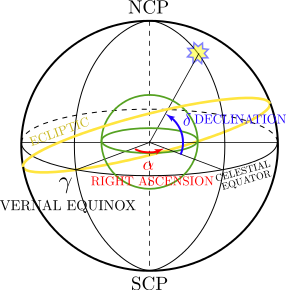
\includegraphics[scale=0.6]{images/equatorial.png}
    \caption{The equatorial coordinates $\alpha$ and $\delta$. The vernal equinox $\gamma$, the equatorial reference point is also depicted. The vernal 
    equinox is the point where the ecliptic (the path the sun traverses over one year) intersects the celestial equator\cite{TEXTBOOK}.}
    \label{fig:equatoral}
\end{figure}
\begin{figure}
    \centering
    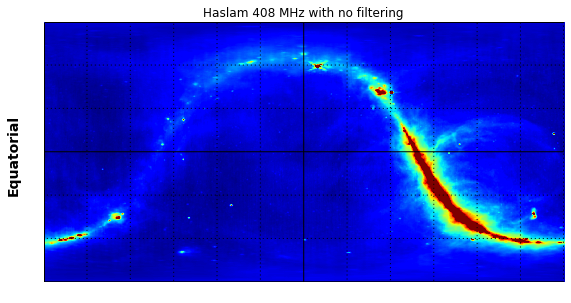
\includegraphics[scale=0.7]{images/UNIVERSEMAP.png}
    \caption{A map of the universe from the perspective of Earth\cite{TEXTBOOK}.}
    \label{fig:universe}
\end{figure}
\FloatBarrier
\subsubsection{Hour Angle and Local Sidereal Time}
The Zenith is the position directly above the observer on the celestial sphere, and similarly the Nadir is the position directly below the observer on the celestial sphere. The local meridian is the hour circle that is formed when the NCP is connected with the Zenith. \\ 
The hour angle of a celestial object is the angular distance between the hour circle of a celestial object and the local meridian in a westerly direction. The hour angle is the time till or since transit and can be used instead of right ascension to keep track of the stars as they move across the celestial sphere. \\
Local sidereal time is a time keeping system that keeps track of the stars, instead of keeping track of the sun, it keeps track of the vernal equinox. The local sidereal time is 4 minutes shorter than the system that keeps track of the sun, the normal solar day.
\subsubsection{Horizontal Coordinates}
In order to determine where a telescope should point on earth in order to observe a source with a specific hour angle, a different coordinate system is needed. The azimuth $\mathcal{A}$ and altitude $\mathcal{E}$ (elevation) is used by an observer on earth to locate an object in the observers sky, the observer's plane is known as the celestial horizon.The azimuth angle is measured in the celestial horizon from due north towards the east, while the altitude of a celestial object is the angle between it and the celestial horizon. Both azimuth and elevation is measured in degrees. The equations for converting between equatorial and horizontal coordinate systems are given below. \begin{eqnarray}
\cos\delta\cos H &=& \cos L_a\sin \mathcal{E} - \sin L_a\cos \mathcal{E}\cos \mathcal{A}\\
-\cos\delta\sin H&=& \cos \mathcal{E}\sin \mathcal{A}\\
\sin\delta &=& \sin L_a\sin \mathcal{E}+\cos L_a \cos \mathcal{E} \cos \mathcal{A} 
\end{eqnarray}
Where $L_a$ denotes latitude.
\subsubsection{Direction Cosine Coordinates}
This coordinate system allows the observer to define their own reference point on the celestial sphere, the point from which all other objects are measured, this reference point is known as the \textit{field center} or \textit{phase center}. \\
There are three coordinates in this system, \textit{l}, \textit{m} and \textit{n}. The equations below are used to convert between the equatorial and direction cosine coordinate systems. 
\begin{eqnarray}
l &=&  \cos \delta  \sin \Delta \alpha \nonumber\\
m &=& \sin \delta \cos \delta_0 - \cos \delta \sin \delta_0 \cos\Delta \alpha \nonumber\\
\delta &=& \sin^{-1}(m\cos \delta_0 + \sin \delta_0\sqrt{1-l^2-m^2})\nonumber\\
\alpha &=& \alpha_0 + \tan^{-1}\bigg(\frac{l}{\cos\delta_0\sqrt{1-l^2-m^2}-m\sin\delta_0}\bigg)\nonumber
\end{eqnarray}
Where $\delta_0$ and $\alpha_0$ are the fundamental reference point of the telescope.
\subsection{Visibility Space}
Interferometry is a powerful technique, it enables us to detect celestial objects and give information on their structure and position. Using aperture synthesis, one can perform synthesis imaging from these measurements\cite{TEXTBOOK}. 
\subsubsection{The Baseline}
The baseline is a separation vector between two antenna in an interferometric array, thus an array can consist of several baselines. The baseline is formed by subtracting the positions of one of the antenna in the array from the position of another antenna in the array. The baseline can be expressed in horizontal coordinates as. \begin{equation}
\mathbf{b}_{\text{ENU}}
=
\lvert \mathbf{b} \rvert
\begin{bmatrix}
\sin \mathcal{A} \cos \mathcal{E}\\
\cos \mathcal{A} \cos \mathcal{E}\\
\sin \mathcal{E}
\end{bmatrix}
\end{equation}
In order to generalise the baseline a new system is needed to map the sky coordinates on the celestial sphere to the baseline. The \textbf{XYZ} system is used for this, this system is defined as follows.
\begin{itemize}
    \item The $X$-axis points towards $(H=0^\textrm{h}, \delta = 0^{\circ})$ 
    \item The $Y$-axis towards $(H=-6^\textrm{h}, \delta = 0^{\circ})$ 
    \item The $Z$-axis towards the NCP.
\end{itemize}
The XYZ coordinates can be calculated using the following:
\begin{equation}
\begin{bmatrix}
X\\Y\\Z
\end{bmatrix}=
\begin{bmatrix}
\lvert \mathbf{b} \rvert \cos \delta \cos H\\
-\lvert \mathbf{b} \rvert \cos \delta \sin H\\
\lvert \mathbf{b} \rvert \sin \delta
\end{bmatrix}
= \lvert \mathbf{b} \rvert
\begin{bmatrix}
\cos L_a \sin \mathcal{E} - \sin L_a \cos \mathcal{E} \cos \mathcal{A}\nonumber\\ 
\cos E \sin \mathcal{A} \nonumber\\
\sin L_a \sin \mathcal{E} + \cos L_a \cos \mathcal{E} \cos \mathcal{A}\\
\end{bmatrix}
\end{equation}
Where $|$\textbf{b}$|$ is the length of the baseline vector, H is the hour angle, $\delta$ is the Declination, $L_a$ is the latitude of the array.
\subsubsection{The u,v,w Space}
Now that the \textbf{XYZ} system is defined, the conversion to the \textit{u,v,w} system is possible. This system is defined below.
\begin{itemize}
    \item The $u$-axis lies in the celestial equatorial plane, and points toward the hour angle $H_0-6^\text{h}$.
    \item The $v$-axis lies in the plane of the great circle with hour angle $H_0$, and points toward the declination $\frac{\pi}{2}-\delta_0$.
    \item The $w$-axis points in the direction of $\mathbf{s_0}$.
\end{itemize}
The conversion from XYZ to uvw is defined as.
\begin{equation}
\begin{bmatrix}
u\\v\\w
\end{bmatrix}=
\begin{bmatrix}
\sin H_0 & \cos H_0 & 0\\ 
-\sin \delta_0 \cos H_0 & \sin\delta_0\sin H_0 & \cos\delta_0\\
\cos \delta_0 \cos H_0 & -\cos\delta_0\sin H_0 & \sin\delta_0\\
\end{bmatrix} 
\begin{bmatrix}
X\\Y\\Z
\end{bmatrix}
\end{equation}
\subsubsection{Visibilities}
The Fourier Transform of the sky brightness distribution is known as the visibility function. An interferometer samples this function. Each baseline pair of the interferometer records one of these samples. The samples received are known as visibilities.
% The interferometer receives a Fourier transform of the image of the sky. This Fourier transform is the visibility function.
% Visibilities are what are received by the interferometer, each baseline receives a visibility and this visibility is used in conjunction with all the others in order to understand the shape of the visibility function and extract information about the sky. 
\subsubsection{UV Tracks and UV Coverage}
Over time, the position of the baseline changes as the earth rotates. This creates a path that is called the UV track of the baseline. If the UV tracks for each baseline are combined together, then the UV coverage is determined. The UV coverage is how much of the UV plane the interferometer is able to cover given its configuration. The visibilities from the baselines are recorded along the UV tracks. 

\subsection{Imaging}
\subsubsection{Aliasing}\label{sec:Aliasing}
Aliasing is an effect that results in misidentification of signals and introduces distortion or errors. It is caused by a sampling rate that is not high enough to properly capture the signal characteristics\cite{aliasing}. The Nyquist Theorem is a theorem that is used to prevent aliasing, it states \textit{The sampling frequency should be at least twice the highest frequency contained in the signal\cite{aliasing}.} In radio interferometry, aliasing can cause the repetition of some signals, so a large enough field of view should always be chosen.

\subsubsection{Gridding}
Gridding is the process of placing the visibilities that have been received by the interferometer and placing them onto a UV plane.\\
The visibilities in the UV plane must be placed onto an image grid which is a two dimensional grid with $N_l \times N_m$ representing the size. Each pixel in the grid has a cell size of $(\Delta \theta_l, \Delta \theta_m)$. The UV tracks are scaled down to the image size which means the the $\Delta u$ and $\Delta v$ are equivalent to the $\Delta l$  and $\Delta m$. This means that the visibilities can be directly applied to the grid. In order to calculate the size of the image from the cell size, the following equation must be applied. 
$$N_l = \frac{\theta_l}{\Delta \theta_l}$$
$$N_m = \frac{\theta_m}{\Delta \theta_m}$$
Where,  $\Delta \theta_l\sim \Delta l$ , $\Delta \theta_m \sim \Delta m$, and $\Delta l = \cos{\Delta \theta_l}$, $\Delta m = \cos{\Delta \theta_m}$. The cell size that is chosen must satisfy the Nyquist theorem in order to avoid aliasing.\\
The visibilities are placed on the grid by convolving the visibilities along the sampling tracks with a function. This is then discretised onto regular points by using a shah function.\\
$V_\text{gridded}[u,v]=[(\mathcal{V}(u,v) \, S(u,v))
\circ C(u,v)] \, III[u,v]$,
where $\mathcal{V}(u,v)$ is the visibility's, $ S(u,v)$ is
the sampling tracks, $C(u,v)$ is the convolution function, and $III[u,v]$ is the shah function.\\
The inverse Fourier Transform can be applied to this grid in order to obtain an image grid, which represents the sky above the interferometer.

\subsubsection{Point Spread Function}
The Point Spread Function, PSF, sometimes referred to as the dirty beam, refers to the response of a
measurement system to a perfect point source at the field center\cite{TEXTBOOK}.
\\
The observed signal of an interferometer is
the convolution of the true signal and the PSF, that is why when imaging the visibilities, point sources
have distortion around them. If a perfect point source were to be imaged, the PSF could clearly be seen for the interferometer that it was applied to. 
The PSF is around all sources in the image, this is because no interferometer is able to observe the entire UV plane without gaps in its observation, errors will be present in the form of the PSF causing distortion around point sources.
